\documentclass[
    iai, % Saisir le nom de l'institut rattaché
    eai, % Saisir le nom de l'orientation
    %confidential, % Décommentez si le travail est confidentiel
]{heig-tb}

%% Choix de la police de caractères
%% (décommenter une des deux lignes suivantes)
%\setmainfont{Latin Modern Roman} % Traditionnel LaTeX
%\setmainfont{TeX Gyre Heros} % Sans sérif

% Police de caractère moins cursive pour le code
% pour une meilleure lisibilité.
\setmonofont{Source Code Pro}

% Générer du texte de remplissage pour les exemples
\usepackage{lipsum}

% Si besoin de gérer des colonnes parallèles
\usepackage{parcolumns}

% Utile pour générer des images temporaires
\usepackage{tikzducks}

% Si besoin d'insérer des formules chimiques
\usepackage{chemfig}
\usepackage[version=4]{mhchem}

\usepackage{pgfplots}
\usepgfplotslibrary{colormaps}
\pgfplotsset{width=10cm,compat=1.18}

\setlength{\fboxsep}{10pt}

\newtheorem{theorem}{Théorème}[section]
\newtheorem{corollary}{Corollaire}[theorem]
\newtheorem{lemma}[theorem]{Lemme}

\usepackage[nooldvoltagedirection,european,americaninductors]{circuitikz}


\signature{mbernasconi.svg} % Remplacer par votre propre signature vectorielle.

\makenomenclature
\makenoidxglossaries
\makeindex

\addbibresource{bibliography.bib}

\newacronym{gcd}{GCD}{Plus grand diviseur commun}
\newacronym{lcm}{LCM}{Plus petit multiple commun}

%% Le glossaire est un élément optionnel qui peut être utile pour expliquer des termes techniques.

\newglossaryentry{heig-vd}{
    name=HEIG-VD,
    description={Haute École d'Ingénierie et de Gestion du canton de Vaud}
}
\newglossaryentry{hes-so}{
    name=HES-SO,
    description={Haute École Supérieure de Suisse Occidentale}
}
\newglossaryentry{latex}{
    name=latex,
    description={Un langage et un système de composition de documents}
}
\newglossaryentry{maths}{
    name=mathematics,
    description={Les mathematiques sont ce que les mathématiciens fonts}
}
% Auteur du document (étudiant-e) en projet de Bachelor
\author{Maria Bernasconi}

% Activer l'option pour l'accord du féminin dans le texte
%\setmale
\setfemale

% Titre de votre travail de Bachelor
\title{Modèle \LaTeX~de rapport de Bachelor}

% Le sous titre est optionnel
\subtitle{Travail de Bachelor}

% Nom du professeur responsable
\teacher {Prof. K.Salimi (HEIG-VD)}

% Mettre à jour avec la date de rendu du travail
\date{\today}

% Numéro de TB
\thesis{7212}


\surroundwithmdframed{minted}

% Utilisé par la nomenclature
\renewcommand\nomgroup[1]{%
  \item[\bfseries
              \ifstrequal{#1}{A}{Constantes physiques}{%
                \ifstrequal{#1}{B}{Groupes}{%
                  \ifstrequal{#1}{C}{Autres Symboles}{}}}%
        ]}

\newcommand{\nomunit}[1]{%
  \renewcommand{\nomentryend}{\hspace*{\fill}#1}}


%% Début du document
\begin{document}
\selectlanguage{french}
\maketitle
\frontmatter
\clearemptydoublepage

%% Requis par les dispositions générales des travaux de Bachelor
%% Le préambule est imposé par la direction de la HEIG-VD.
%% Le texte ne doit pas être modifié.

\chapter*{Préambule}
\addcontentsline{toc}{chapter}{Préambule}

Ce travail de Bachelor (ci-après \textbf{TB}) est réalisé en fin de cursus d'études, en vue de l'obtention du titre de Bachelor of Science HES-SO en \thefield.

En tant que travail académique, son contenu, sans préjuger de sa valeur, n'engage ni la responsabilité de l'auteur, ni celles du jury du travail de Bachelor et de l'École.

Toute utilisation, même partielle, de ce TB doit être faite dans le respect du droit d'auteur.

\vskip 4em%
    {\leftskip8cm\relax
        HEIG-VD \\
        Le Chef du Département\par
        \vfil
    }
Yverdon-les-Bains, le \thedate

%% L'authentification est imposée par la direction de la HEIG-VD.
%% Le texte ne doit pas être modifié.

\chapter*{Authentification}
\addcontentsline{toc}{chapter}{Authentification}

Je soussigné\ifx\thegenre\female e\fi, \theauthor, atteste par la présente avoir réalisé seul\ifx\thegenre\female e\fi~ce travail et n'avoir utilisé aucune autre source que celles expressément mentionnées.

\vfil
{\leftskip9cm\relax\theauthor\par
    \ifdefined\thesignature
        %\hspace{8cm}
        \printsignature

    \fi
}
\vfil
Yverdon-les-Bains, le \thedate

%% Une préface est optionnelle
\chapter*{Préface}
\addcontentsline{toc}{chapter}{Préface}

Ce document constitue un modèle officiel de document \LaTeX{} élaboré par la Haute École d'Ingénierie et de Gestion du Canton de Vaud (HEIG-VD) à l'intention de ses étudiantes et étudiants. Il a été conçu dans le but de faciliter la rédaction des travaux de Bachelor en offrant une base solide et structurée, respectant les standards académiques en vigueur.

Ce modèle ne se limite pas à un simple cadre formel ; il intègre également des recommandations pratiques et des exemples concrets destinés à guider les utilisateurs tout au long du processus de rédaction. La structure proposée, bien que recommandée pour des raisons pédagogiques, reste souple et adaptable selon les besoins spécifiques de chaque projet. Elle vise avant tout à offrir un appui méthodologique pour développer un travail cohérent et rigoureux.

Les annexes jointes apportent un éclairage supplémentaire sur divers aspects relatif à ce modèle et son utilisation. Elles couvrent des sujets allant de la rédaction des contenus à la justification des choix techniques, en passant par des conseils liés à la mise en page et à l'exploitation optimale du modèle proposé.

Nous espérons que ce modèle saura accompagner efficacement chaque étudiante et chaque étudiant dans la réalisation de ses travaux et contribuer à l'excellence des productions académiques au sein de la HEIG-VD.


%% Résumé / Résumé publiable / Version abrégée
\begin{abstract}
  %% Le résumé du projet doit:
%% 1. Être rédigé dans la langue du rapport
%% 2. Optionnellement offrir une traduction anglaise
%% 3. Être court, concis et informatif (entre 150-300 mots)
%% 4. Être rédigé en un seul paragraphe, sans mise en forme (gras ou italique)
%% 5. Être au passé (le projet étant terminé, on résume ce qui a été fait et les résultats obtenus)

% Francais
\lipsum[1]

%% L'asterisme est un signe typographique en forme d'étoile, utilisé pour marquer une pause dans un texte ou pour séparer des paragraphes. Il est souvent utilisé pour indiquer un changement de scène dans un récit. Bien qu'il se fasse rare dans la typographie moderne, c'est un symbole de choix pour séparer les différentes langues du résumé de thèse.
\asterism

% English
\lipsum[3]

\end{abstract}

%% Sommaire et tables
\clearemptydoublepage
{
  \tableofcontents
  \let\cleardoublepage\clearpage
  \listoffigures
  \let\cleardoublepage\clearpage
  \listoftables
  \let\cleardoublepage\clearpage
  \listoflistings
}

\printnomenclature
\clearemptydoublepage
\pagenumbering{arabic}

%% Contenu
\mainmatter

\chapter{Introduction}

L'introduction est une section \emph{obligatoire} dans un rapport technique. Elle contient généralement au moins quatre paragraphes répondant aux questions suivantes: quel est le problème à résoudre ? Pourquoi y a-t-il un problème ? Quelle est la solution envisagée ? Pourquoi est-ce que la solution envisagée est meilleure que l'état de l'art ?

En bref, on vous demande d'introduire votre travail, l'idée de départ et les objectifs attendus. Le lecteur qui découvrirait votre projet au travers de cette introduction devrait ainsi être capable d'en comprendre le cadre, l'idée générale et les aboutissants du projet.

\section{Contexte}

Cette section \emph{n'est pas obligatoire}, mais elle est souvent présente en préambule de l'introduction afin de préciser le contexte du travail \cad et le cadre formel dans lequel le travail est mené. Dans bien des cas, le projet est réalisé dans un contexte industriel, vis-à-vis d'une problématique un peu en marge avec l'intitulé du projet. Le contexte permet de clarifier les enjeux et les contraintes du projet.

\section{Problématique}

La problématique est le cœur de l'introduction. Elle doit être clairement formulée et doit permettre de comprendre le problème que vous vous apprêtez à résoudre. Il est important de bien définir le problème pour que le lecteur puisse comprendre les enjeux du projet et les raisons pour lesquelles vous avez choisi de travailler sur ce sujet et pourquoi vous y amenez une valeur ajoutée.

\section{Objectifs}

On attend généralement une liste d'objectifs clairs et précis. Cette liste doit être cohérente avec le contexte et les enjeux du projet. Les objectifs doivent être mesurables et atteignables. Ils doivent être formulés de manière à ce qu'ils puissent être validés à la fin du projet.

\section{Méthodologie}

Vous pouvez ajouter une section méthodologie expliquant votre démarche pour atteindre les objectifs. Cette section peut être utile pour expliquer les choix que vous avez faits, les outils que vous avez utilisés, les raisons pour lesquelles vous avez choisi une approche plutôt qu'une autre.

\chapter{État de l'art}

L'état de l'art présente une revue de la littérature sur le sujet de votre travail. Il s'agit de présenter les travaux antérieurs qui ont été réalisés sur le sujet, les solutions existantes, les technologies utilisées, les méthodes employées, les résultats obtenus, etc. L'état de l'art permet de situer votre travail par rapport à ce qui a déjà été fait et de justifier l'originalité de votre approche.

\section{Travaux existants}

Dans cette section, vous pourriez présenter les travaux existants qui ont été réalisés sur le sujet de votre travail. Vous pourriez les classer par thème, par auteur, par date, etc. N'oubliez pas que vous devez citer les sources de manière précise et les référencer dans la bibliographie.

\section{Technologies et méthodes existantes}

Dans cette section, vous pourriez présenter les technologies et les méthodes connues qui ont été utilisées pour résoudre le problème que vous vous apprêtez à résoudre. Vous pourriez les comparer, les évaluer, les critiquer, etc. N'oubliez pas que vous devez citer les sources de manière précise et les référencer dans la bibliographie.

L'objectif n'est pas de faire un cours magistral sur le sujet, mais de donner un aperçu des connaissances existantes sur le sujet qui servent le propos que vous vous apprêtez à développer. Il peut être utile de présenter des tableaux comparatifs, des graphiques, des schémas, etc.

Évitez d'aller à la pioche de figures trop détaillées sur internet. N'hésitez pas à les dessiner vous-même pour les adapter à votre propos. N'oubliez pas que vous racontez une histoire, vous posez peu à peu les bases de votre raisonnement et vous amenez le lecteur saisir les éléments clés qui lui permettront de comprendre au fil de la lecture votre travail.
\chapter{Implémentation}

Ce chapitre est dédié à la description de l'implémentation du projet, c'est là que vous décrivez comment vous avez réalisé votre projet, comment vous avez mené vos expériences.

Présentez votre conception à l'ade de schémas, de diagrammes. Expliquez votre architecture logicielle, votre conception électronique, vos analyses de données, etc.

Scindez ce chapitre en plusieurs sections si nécessaire. Si votre projet est multidisciplinaire, vous pouvez par exemple avoir une section pour l'implémentation logicielle et une autre pour l'implémentation matérielle.
\chapter{Analyse des résultats}

Vous avez réalisé votre projet, vous avez mené vos expériences, vous avez collecté vos données, vous avez analysé vos résultats. Il est temps de les présenter et de les interpréter. Cette section est cruciale pour la validation de votre travail. Vous devez montrer que vous avez atteint vos objectifs, que vous avez répondu à vos questions de recherche, que vous avez résolu le problème que vous vous étiez fixé.

Prenez garde à ne pas surcharger votre rapport de données brutes qui ne servent pas l'objectif final de votre projet. Avec tout le temps que vous avez passé sur votre projet, vous avez probablement collecté une quantité impressionnante de données, mais la plupart n'ont d'importance que parce que vous les avez collectées. Vous devez sélectionner les données qui sont pertinentes.

\section{Présentation des résultats}

Généralement on commence par présenter les résultats de manière synthétique. Vous pouvez utiliser des tableaux, des graphiques, des schémas, des figures, des photos, des extraits de code, etc., pour illustrer vos résultats. Vous devez les commenter, les expliquer, les interpréter.

Pensez à aux unités, aux biais, aux incertitudes.

\section{Discussion des résultats}

Dans un second temps, vous pouvez discuter vos résultats. Vous pouvez les comparer à ceux de la littérature, les évaluer, les critiquer, les justifier. Vous pouvez expliquer pourquoi vous avez obtenu ces résultats, pourquoi ils sont pertinents.

\chapter{Conclusion}

On dénote deux types de conclusion : la conclusion technique et la conclusion personnelle. La conclusion est la deuxième partie qui sera lue par un manager de société après le résumé. Elle doit être concise et claire. Elle doit résumer les résultats obtenus et dresser une conclusion objective du projet. La conclusion technique doit être basée sur les résultats obtenus et doit être en lien avec les objectifs fixés. La conclusion personnelle est une réflexion personnelle sur le projet. Elle peut contenir des éléments qui n'ont pas été abordés dans le rapport, des éléments qui ont été appris durant le projet, des éléments qui ont été appréciés ou non, etc.

Bien entendu vous pouvez également donner un sens plus intime en parlant de votre ressenti, de ce que vous avez appris, de ce que vous avez aimé ou non, etc. C'est une manière de donner une touche personnelle à votre travail.

Il peut être coutume de signer la conclusion encore que votre rapport comporte déjà votre signature numérique. Cela reste un choix personnel.

\vfil
\hspace{8cm}\makeatletter\@author\makeatother\par
\hspace{8cm}\begin{minipage}{5cm}
    % Place pour signature numérique
    \printsignature
\end{minipage}

\clearpage
\printbibliography

\appendix
\appendixpage
\addappheadtotoc

\chapter{C'est quoi une annexe ?}

Précisons-le tout de toute, les annexes ne possèdent pas de contenu \underline{normatif} mais \underline{descriptif}. Tout contenu annexé ne doit pas être indispensable à la compréhension du travail réalisé, elles sont ajoutées en complément du rapport.

Les annexes contiennent généralement :

\begin{itemize}
    \item les dessins mécaniques (mises en plan);
    \item les schémas électriques détaillés;
    \item des photographies du projet;
    \item des scripts et des extraits de code source;
    \item des documents techniques \pex \emph{datasheet};
    \item des développements mathématiques.
\end{itemize}

Les annexes sont utiles pour reproduire le travail réalisé, pour le comprendre en profondeur.

Il est courant d'avoir plusieurs annexes, chacune étant numérotée et identifiée par une lettre.

Évitez également d'être trop généreux dans vos annexes, elles ne doivent pas être un fourre-tout et il peut être mal vu d'avoir un rapport de 50 pages avec 200 pages d'annexes. Préférez des ressources en lignes, mentionnez vos sources, vos dépôts de code (GitHub, GitLab, Bitbucket, etc.). Profitez de donner les hash de vos commits pour que le lecteur puisse retrouver exactement la version de votre code source utilisée au moment de la rédaction du rapport.
\chapter{Exemples}

Ce chapitre est dédié à la présentation de quelques exemples de contenu que vous pourriez intégrer dans votre rapport. Il est important de noter que ce document est un modèle et que vous devriez adapter son contenu à votre projet. Les exemples suivants sont bien entendu donnés à titre indicatif.

\section{Citations et bibliographie}

Citer vos sources est essentiel. Avec \texttt{biblatex} vous pouvez facilement citer des articles, des livres ou des sites internet. Toutes les citations dans le texte seront automatiquement regroupées en fin de document dans la section \guillemotleft{} Bibliographie\guillemotright.

À titre d'exemple nous pouvons citer un article d'Einstein \cite{einstein} ou le livre de Dirac \cite{dirac}. La communauté scientifique à de nombreux consensus pour référencer les articles scientifiques. On parle du style des citations. Certains styles sont normalisés comme le style \texttt{IEEEtran} ou \texttt{APA}. Le style \texttt{IEEEtran} est souvent utilisé pour les articles scientifiques en ingénierie et en informatique. Le style \texttt{APA} est souvent utilisé en psychologie et en sciences sociales. Avec \LaTeX{} vous pouvez facilement changer le style de citation en modifiant l'option \mintinline{latex}|style=alphabetic| dans le fichier \texttt{heig-tb.cls}.

Ne citez pas pour citer, mais citez pour appuyer vos arguments sur des travaux existants. Elles doivent être utilisées pour montrer que vous avez fait des recherches sur le sujet.

Parfois il peut être utile d'utiliser un gestionnaire de bibliographie. La communauté académique recommande l'outil \href{https://www.zotero.org/}{Zotero} qui permet de gérer une bibliothèque numérique d'ouvrages et de références numériques. Il permet également de générer une bibliographie compatible avec \LaTeX.

Notez qu'il est très facile d'obtenir l'extrait \texttt{bibtex} depuis des journaux. Sélectionnez \emph{export/citation}. Si vous le pouvez, choisissez \texttt{bibtex}. Dans le cas d'un format \texttt{.ris}, utilisez un convertisseur en ligne comme \href{http://www.bruot.org/ris2bib/}{ris2bib}.

\section{Mathématiques}

L'une des principales forces de \LaTeX{} est la saisie d'équations. L'équation \ref{eq:1}, citée à titre d'exemple, représente la transformation de phase d'une lentille biconvexe. Pour rédiger une équation \LaTeX{} vous pouvez utiliser des outils en ligne tels que \href{https://www.latex4technics.com/}{latex4technics}. Essayez autant que possible d'écrire vos équations à la main.
La courbe d'apprentissage n'est pas très raide et la valeur ajoutée est grande. Vous pouvez vous aider du panneau de \LaTeX{} Workshop dans Visual Studio Code. Il est accessible via le raccourci clavier \keystroke{Ctrl} + \keystroke{Alt} + \keystroke{X}.

\begin{equation} \label{eq:1}
    \begin{split}
        L(x,y) & = \exp\left( - i\frac{{2\pi }}{\lambda }\left( {n\Delta \varphi (x,y) + \Delta {\varphi _0} - \Delta \varphi (x,y)} \right)\right)     \\
               & = {\exp\left({i\frac{{2\pi }}{\lambda }\Delta {\varphi _0}}\right)}{\exp\left({ - i\frac{{2\pi }}{{\lambda f}}({x^2} + {y^2})}\right)}
    \end{split}
\end{equation}

Pensez à numéroter vos équations pour pouvoir les citer dans le texte.

\subsection{Formules avec explications}

L'exemple suivant montre les quatre équations de Maxwell sous forme différentielle à gauche et intégrales à droite. Les constantes sont expliquées après l'équation.

\begin{subequations}
    \begin{align}
        \nabla \cdot \vec{E}  & = \frac{\rho}{\varepsilon_0}                                              & \oint_{S} \vec{E} \cdot d\vec{A} & = \frac{1}{\varepsilon_0} \int_{V} \rho \, dV                                                              \\[1em]
        \nabla \cdot \vec{B}  & = 0                                                                       & \oint_{S} \vec{B} \cdot d\vec{A} & = 0                                                                                                        \\[1em]
        \nabla \times \vec{E} & = -\frac{\partial \vec{B}}{\partial t}                                    & \oint_{C} \vec{E} \cdot d\vec{l} & = -\frac{d}{dt} \int_{S} \vec{B} \cdot d\vec{A}                                                            \\[1em]
        \nabla \times \vec{B} & = \mu_0 \vec{J} + \mu_0 \varepsilon_0 \frac{\partial \vec{E}}{\partial t} & \oint_{C} \vec{B} \cdot d\vec{l} & = \mu_0 \int_{S} \vec{J} \cdot d\vec{A} + \mu_0 \varepsilon_0 \frac{d}{dt} \int_{S} \vec{E} \cdot d\vec{A}
    \end{align}
\end{subequations}

\vspace{1em}

où :

\begin{tabular}{rll}
    $\varepsilon_0$ & permittivité du vide & \si{\farad\per\meter}          \\
    $\mu_0$         & perméabilité du vide & \si{\henry\per\meter}          \\
    $\rho$          & densité de charge    & \si{\coulomb\per\meter\cubed}  \\
    $\vec{J}$       & densité de courant   & \si{\ampere\per\meter\squared} \\
    $\vec{E}$       & champ électrique     & \si{\volt\per\meter}           \\
    $\vec{B}$       & champ magnétique     & \si{\tesla}                    \\
\end{tabular}

\subsection{Encadrés mathématiques}

Souvent on veut mettre en évidence une équation en l'encadrant. C'est possible avec \verb!fbox!. Voici l'exemple avec l'équation de Schrödinger \eqref{eq:schrodinger}:

\begin{equation}
    \begin{ceqn}
        \fbox{$i\hbar \frac{\partial}{\partial t} \Psi(\vec{r},t) = \left[ -\frac{\hbar^2}{2m} \nabla^2 + V(\vec{r},t) \right] \Psi(\vec{r},t)$}
        \label{eq:schrodinger}
    \end{ceqn}
\end{equation}

\subsection{Théorèmes et définitions}

\LaTeX{} permet nativement de définir des théorèmes, des lemmes, des corollaires, des définitions, etc. Ces environnements sont très utiles pour structurer votre document. Voici quelques exemples :

\begin{theorem}
    Soit \(f\) une fonction dont la dérivée existe en tout point, alors \(f\) est
    une fonction continue.
\end{theorem}

\begin{theorem}[Théorème de Pythagore]
    \label{pythagorean}
    Ceci est un théorème concernant les triangles rectangles et peut être résumé par l'équation suivante :
    \[ x^2 + y^2 = z^2 \]
\end{theorem}

Une conséquence du théorème \ref{pythagorean} est l'énoncé du corollaire suivant.

\begin{corollary}
    Il n'existe pas de triangle rectangle dont les côtés mesurent 3 cm, 4 cm et 6 cm.
\end{corollary}

Vous pouvez référencer des théorèmes tels que \ref{pythagorean} lorsqu'une étiquette est attribuée.

\begin{lemma}
    Étant donnés deux segments de droite de longueurs respectives \(a\) et \(b\), il existe un
    nombre réel \(r\) tel que \(b = ra\).
\end{lemma}


\section{Diagrammes}

Les diagrammes de flux peuvent être réalisés en utilisant l'outil \href{https://app.diagrams.net/}{draw.io}. Une exportation en \texttt{.drawio} (non compressé) permet de garder les sources de la figure. Le rendu en \texttt{.pdf} sera réalisé à la volée à la compilation ce qui est l'intérêt principal d'utiliser ce modèle.

L'objectif est d'avoir qu'une source de vérité \cad pas d'image intermédiaire à stocker, et réduire la quantité d'information dans votre dépôt GitHub.

Puisque la source de ces diagrammes est au format XML, les textes sont accessibles au correcteur orthographique et il vous est rendu possible les modifier sans avoir à éditer l'image. La figure \ref{euclide.drawio} en est un exemple.

\fig[H, width=9cm]{Algorithme d'Euclide}{euclide.drawio}

Notons qu'il est inutile d'insérer des images coloriées là où la couleur n'offre aucune valeur ajoutée ; évitez également les ombrages et autres effets de style. Enfin, préférez toujours des représentations vectorielles là où c'est possible.

Voici un autre type de diagramme utile (figure \ref{sequence.drawio}), celui d'une séquence UML.

\fig[H, width=0.6\textwidth]{Diagramme de séquence}{sequence.drawio}

Ce modèle apporte la commande \verb!\fig! qui peut prendre plusieurs options. Utilisez \verb!H! pour forcer la figure à apparaître à l'endroit de la déclaration. Ajustez la largeur de la figure à \SI{80}{\percent} de largeur de page avec \verb!width=0.8\textwidth!.

\section{Figures}

Pour présenter vos résultats d'expérience, vous pouvez soit dessiner des graphiques manuellement en utilisant des outils de dessin vectoriel comme Inkscape ou Adobe Illustrator, comme illustré à la figure \ref{plot.svg}.

\fig[H, width=1\textwidth]{Exemple de graphique plan}{plot.svg}

Vous pouvez utiliser Python ou Matlab pour générer des figures à la volée à partir d'une source de données. À titre d'exemple, le code source \ref{python} permet de générer la figure \ref{bode.py}.
\begin{listing}[ht]
    \inputminted{python}{assets/figures/bode.py}
    \caption{Génération d'un diagramme de Bode \label{python}}
\end{listing}

\fig[H, width=12cm]{Diagramme de Bode généré à la volée}{bode.py}

\subsection{Sous figures}

Vous pouvez insérer des sous-figures, par exemple ici 4 figures côte à côte (2 colonnes et deux lignes). Les images sont remplacées par \verb!\tikz\randuck! permettant de générer un canard aléatoire à chaque compilation.

\begin{figure}[H]
    \centering
    \begin{subfigure}{0.45\textwidth}
        \centering
        
\begin{tikzpicture}
            \randuck
        \end{tikzpicture}
        \caption{Canard 1}
    \end{subfigure}
    \begin{subfigure}{0.45\textwidth}
        \centering
        
\begin{tikzpicture}
            \randuck
        \end{tikzpicture}
        \caption{Canard 2}
    \end{subfigure}

    \begin{subfigure}{0.45\textwidth}
        \centering
        
\begin{tikzpicture}
            \randuck
        \end{tikzpicture}
        \caption{Canard 3}
    \end{subfigure}
    \begin{subfigure}{0.45\textwidth}
        \centering
        
\begin{tikzpicture}
            \randuck
        \end{tikzpicture}
        \caption{Canard 4}
    \end{subfigure}
    \caption{Quatre canards}
\end{figure}

\subsection{Dessins techniques}
La présentation de dessins mécaniques est préférée en vue filaire. SolidWorks conserve la représentation vectorielle à l'exportation, mais pas lorsqu'il y a des textures ou des rendus. À partir du PDF généré, l'image peut être isolée et sauvegardée en format SVG.

\begin{figure}[!ht]
    \begin{center}
        \includegraphics[width=10cm]{\assetsdir/assembly.svg.pdf}
    \end{center}
    \caption[Assemblage mécanique]{\label{assembly}Réducteur cycloïdal de puissance comportant 6. l'axe de sortie, 14. le roulement de sortie, 1. le corps du réducteur en aluminium, 3 et 5. les disques cycloïdaux et 2. les goupilles de prise... D'autres informations liées à la figure elle-même peuvent aussi figurer dans la légende.}
\end{figure}

Notez ici que la légende est particulièrement longue. Celle que vous retrouverez dans la table de figures est plus courte. La commande \mintinline{latex}{\caption[courte]{longue}} permet de saisir une légende courte pour la table des figures et une légende longue pour documenter la figure. Utilisez \mintinline{latex}{\fig[short=Légende courte]{Légende longue}{fichier}}.

La figure \ref{assembly} est un dessin technique épuré qui permet de décrire un phénomène ou un fonctionnement important dans le rapport technique. Les mises en plan détaillées seront quant à elles disponibles en annexes.

\section{Formules chimiques}

Pour les formules chimiques, utilisez le paquet \texttt{mhchem}. Par exemple, l'équation \ref{eq:2} représente la réaction de combustion du méthane.

\begin{figure}[ht]
    \begin{center}
        \chemfig{A*6(-B=C(-CH_3)-D-E-F(=G)=)}
    \end{center}
    \caption{Formule chimique \label{fig:chem}}
\end{figure}

\begin{equation} \label{eq:2}
    \ce{CH4 + 2O2 -> CO2 + 2H2O}
\end{equation}

\newpage
\section{Tableaux}

Concernant les tableaux un seul conseil : restez simple et minimaliste, n'ajoutez des séparateurs que là ou c'est nécessaire pour améliorer la lisibilité. Une liste de quelques cantons suisses est donnée à titre d'exemple dans la table \ref{cantons}.

\begin{table}[ht]
    \begin{center}
        \caption{Liste des cantons \label{cantons}}
        \begin{tabular}{rlr}
            \toprule
            Abréviation & Nom du canton & Depuis                  \\
            \midrule
            ZH          & Zürich        & \ordinalnum{1} mai 1351 \\
            FR          & Fribourg      & 22 décembre 1481        \\
            VD          & Vaud          & 19 février 1815         \\
            VS          & Valais        & 4 août 1815             \\
            NE          & Neuchâtel     & 19 mai 1815             \\
            GE          & Genève        & 19 mai 1815             \\
            \bottomrule
        \end{tabular}
    \end{center}
\end{table}

Comparez la lisibilité de cette même table avec celle que vous pourriez trouver dans un document Word. Évitez par conséquent les bordures et les couleurs.

\begin{table}[ht]
    \begin{center}
        \caption{Liste des cantons (vilain)}
        \begin{tabular}{|l|l|l|} \hline
            \textbf{Abréviation} & \textbf{Nom du canton} & \textbf{Depuis}         \\
            \Xhline{4\arrayrulewidth}
            ZH                   & Zürich                 & \ordinalnum{1} mai 1351 \\ \hline
            FR                   & Fribourg               & 22 décembre 1481        \\ \hline
            VD                   & Vaud                   & 19 février 1815         \\ \hline
            VS                   & Valais                 & 4 août 1815             \\ \hline
            NE                   & Neuchâtel              & 19 mai 1815             \\ \hline
            GE                   & Genève                 & 19 mai 1815             \\ \hline
        \end{tabular}
    \end{center}
\end{table}

\subsection{Exigences techniques}

Si vous devez donner une spécification technique, n'oubliez pas de mentionner les valeurs minimales, maximales et nominales sans omettre l'unité de mesure. Notez que les séparateurs verticaux sont souvent critiqués pour réduire la lisibilité, mais parfois ils sont utiles. Utilisez-les avec parcimonie. Jouez avec l'alignement des colonnes pour accroître la lisibilité et utilisez l'environnement \mintinline{latex}{tabularx} pour plus d'unité dans les largeurs de vos tableaux.

\begin{table}[ht]
    \begin{center}
        \caption{Exigences techniques \label{specification}}
        \begin{tabularx}{\textwidth}{cXcccr}
            \toprule
            No. & Exigence                                                                   & Min. & Nom. & Max. & Unité                           \\
            \midrule
            E1  & Tension d'alimentation                                                     & 12   & 24   & 48   & \si{\volt}                      \\
            E2  & Fréquence                                                                  & 50   &      & 60   & \si{\hertz}                     \\
            E3  & Concentration                                                              &      & 300  & 1200 & \si{\nano\gram\per\milli\litre} \\
            E4  & \multicolumn{5}{l}{Doit pouvoir être stoppé à l'aide d'un arrêt d'urgence}                                                        \\
            \bottomrule
        \end{tabularx}
    \end{center}
\end{table}

L'exemple de la table \ref{specification}, assigne pour chaque exigence un numéro unique. Cette table est \textbf{normative}, chaque élément doit pouvoir être référencé par un identifiant unique (cf. T\ref{specification}-E3). Dans le cas où cet identifiant est utilisé en dehors de ce document, la version du document devra être renseignée.

\section{Annotations et références}

\subsection{Index}
\LaTeX{} permet d'indexer les mots \index{mots} importants. Il suffit de placer les termes importants d'un paragraphe dans la commande \mintinline{latex}{\index{terme}} et ils apparaîtront automatiquement à la fin de ce rapport dans l'index du document. L'intérêt réside principalement dans une version imprimée. Si votre rapport n'est pas destiné à être imprimé, l'index n'est pas nécessaire.

\index{Napoléon}

Imaginons que dans cette section nous parlions du cheval blanc \index{cheval blanc} de Napoléon. Il se pourrait que le lecteur recherche ce passage dans la version imprimée du rapport. Avec l'index, rien de plus facile. Allez jeter un œil à la page \pageref{index}.

\subsection{Notes maginales}

\maraja{Je suis une marginale, et je suis utile pour résumé un paragraphe en quelques mots.} Vous pouvez sporadiquement utiliser les notes maginales pour mettre en exergue un point important. Elles sont particulièrement utiles pour résumer un paragraphe en quelques mots. Elles sont également utiles pour ajouter des commentaires ou des réflexions personnelles.

\subsection{Notes de bas de page}

Parfois, il est plus élégant d'annoter une définition en utilisant une note de bas de page \footnote{La note en bas de page (ou note de bas de page) est une forme littéraire, consistant en une ou plusieurs lignes ne figurant pas dans le texte.}.

\section{Glossaire et acronymes}

La \Gls{heig-vd} membre de la \Gls{hes-so} propose ce modèle de document. Le format \LaTeX~est particulièrement adapté pour les documents qui contiennent des expressions mathématiques. Pour plus de détail sur l'utilisation d'un glossaire, se référer à \href{https://www.overleaf.com/learn/latex/Glossaries}{Overleaf/Glossaires}. Tiens donc, ci-dessus, nous utilisons deux acronymes. Les trouverez-vous dans le glossaire en page \pageref{glossaire} ?

\section{Unités de mesure}

Le plus difficile dans la rédaction d'un rapport technique est de rester cohérent dans l'utilisation des unités de mesure. Contrairement aux idées reçues les unités ne sont pas placées entre crochets ni mises en italiques.

Une espace fine doit être placée entre le nombre et l'unité, et on évitera les barres de division pour les unités composées.

Le paquet \texttt{siunitx} facilite grandement la saisie de quantités. La commande suivante permet d'afficher par exemple \qty{42.12}{\kilo\gram\metre\per\square\second}.\par

\mintinline{text}{\qty{42.12}{\kilo\gram\metre\per\square\second}}\par

Pour afficher simplement une unité comme le \si{\kilo\gram} on utilise la commande \mintinline{text}{\si{\kilo\gram}}.

\section{Mise en forme}

\subsection{Multi-colonnes}

Si vous avez de longues listes, ou pour certains paragraphes, il peut être utile d'utiliser l'environnement \verb|\multicols| pour afficher le texte sur plusieurs colonnes. Cela permet de gagner de la place et d'améliorer la lisibilité. Par exemple, voici un extrait de l'article de la Constitution fédérale suisse de 1999.

\begin{multicols}{2}
    \begin{enumerate}
        \item La Confédération et les cantons veillent à ce que les enfants et les jeunes soient protégés contre la négligence et la violence, contre l'exploitation et la discrimination et qu'ils puissent se développer de manière saine.
        \item Ils veillent à ce que les enfants et les jeunes puissent exercer leurs droits et assumer leurs responsabilités.
        \item Ils encouragent les parents à assumer leur rôle d'éducateurs et leur apportent leur soutien.
        \item Ils tiennent compte des intérêts de l'enfant lorsqu'ils prennent des décisions qui le concernent.
        \item Ils veillent à ce que les enfants et les jeunes soient informés de leurs droits et de leurs devoirs.
        \item Ils encouragent les institutions et les organisations qui s'engagent en faveur de l'enfance et de la jeunesse.
    \end{enumerate}
\end{multicols}

\subsection{Colonnes parallèles}

\maraja{Un pangramme est une phrase contenant toutes les lettres de l'alphabet.}Le module \verb!parcolumns! permet de créer des colonnes parallèles. Cela peut être utile pour comparer des textes en plusieurs langues ou pour afficher des traductions. Voici un exemple de \emph{pangramme} en différentes langues.\par

\begin{parcolumns}{4}
    \colchunk{Le vif zéphyr jubile sur les kumquats du clown gracieux.}
    \colchunk{The quick brown fox jumps over the lazy dog.}
    \colchunk{Victor jagt zwölf Boxkämpfer quer über den großen Sylter Deich.}
    \colchunk{Quel fez sghembo copre davanti.}
\end{parcolumns}

\subsection{Boîtes colorées}

\maraja{Les boîtes disponibles sont: note, info, tip, success, warning, important, hint, bug, example} Il est parfois utile de mettre en évidence certaines parties, pour indiquer une astuce, un point important, un exemple, etc. Voici quelques exemples mais un conseil, n'en abusez pas.

\begin{callout}[callout tip]
    \lipsum[1][1]
\end{callout}

\begin{callout}[callout info]
    \lipsum[1][2]
\end{callout}

\begin{callout}[callout success]
    \lipsum[1][3]
\end{callout}

\begin{callout}[callout warning]
    \lipsum[1][4]
\end{callout}

\section{Code source}

Ce modèle vous offre deux environnements pour afficher du code source. Le plus traditionnel est l'environnement Listing et le second est l'environnement Minted. Le premier est plus simple à utiliser, mais le second offre une coloration syntaxique plus précise et utilise Python comme backend pour la coloration syntaxique.

\begin{listing}[ht]
    \inputminted{c}{assets/code/fibonacci.c}
    \caption{Exemple de programme en C \label{cminted} avec Minted}
\end{listing}

\begin{listing}[ht]
    \lstinputlisting{assets/code/fibonacci.c}
    \caption{Exemple de programme en C \label{clist} avec Listing}
\end{listing}

Voici un exemple directement dans le texte :

\begin{minted}{python}
def hello_world():
print("Hello, world!")
\end{minted}

\clearpage
\section{Tikz}

Ti\textit{k}Z est un outil puissant pour dessiner des graphiques en \LaTeX. Il est particulièrement utile pour les diagrammes de circuits, les graphiques 2D et 3D, les diagrammes de séquence, les arbres, etc. Voici un exemple simple de diagramme de séquence. On préfèrera aujourd'hui des outils WYSIWYG comme draw.io pour les diagrammes mais pour des diagrammes techniques de haute qualité, Tikz reste un outil de choix. Sa courbe d'apprentissage est raide, mais les résultats sont impressionnants.

N'hésitez pas à vous inspirer d'exemples disponibles sur internet (\href{https://texample.net/category/science-technology/}{texample.net}).

\subsection{PGF Plots}

PGF Plots est un package TikZ spécialisé dans les graphiques. Voici l'exemple d'un graphique 3D réalisé avec PGF Plots. Il est également possible de générer des graphiques à partir de données tabulaires. Pour plus d'informations, consultez la documentation de PGF Plots.

\begin{figure}[H]
    \centering
    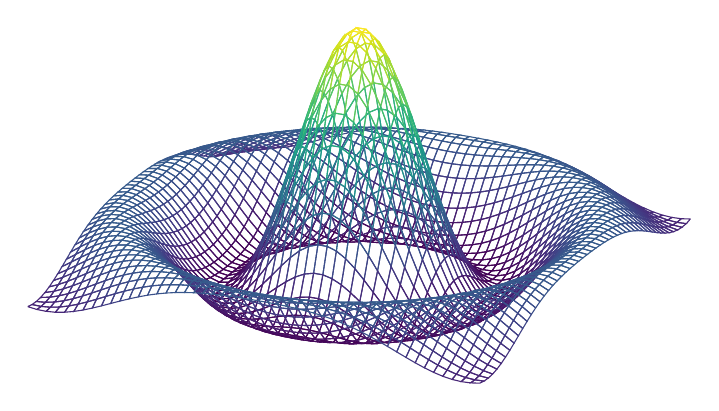
\begin{tikzpicture}
        \begin{axis}[
                hide axis,
                colormap/viridis,
            ]
            \addplot3[
                mesh,
                samples=50,
                domain=-8:8,
            ]
            {sin(deg(sqrt(x^2+y^2)))/sqrt(x^2+y^2)};
            %\addlegendentry{\(\frac{sin(r)}{r}\)}
        \end{axis}
    \end{tikzpicture}
    \caption{Exemple de graphique 3D avec PGF Plots}
\end{figure}

\subsection{Jonction semiconducteur}

Voici un autre exemple d'un diagramme de jonction semi-conducteur.

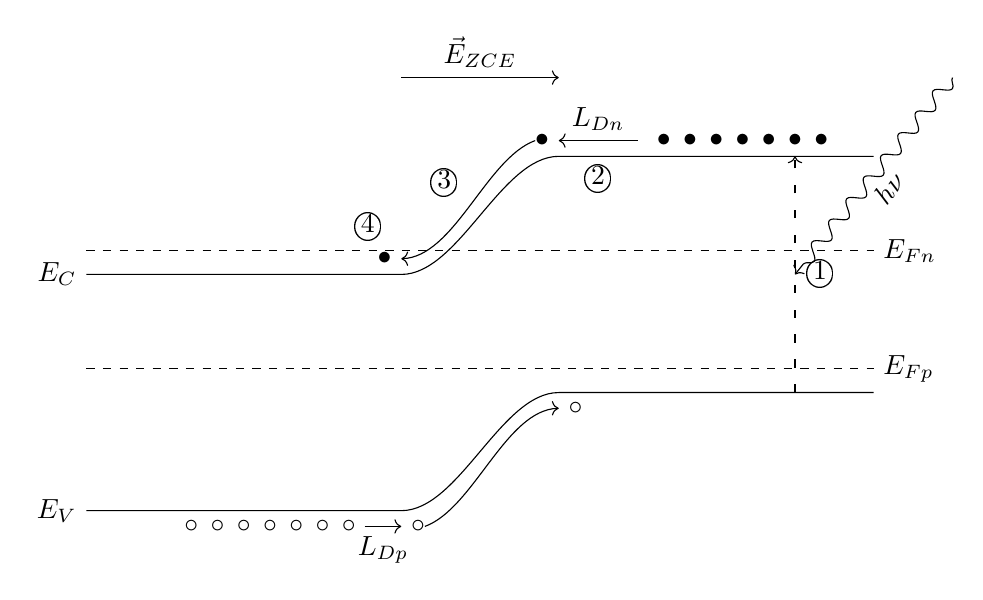
\begin{tikzpicture}
    % variables for pn-junction diagram:
    % all parameters are in tikz scale
    % p-side of the junction is here on the right

    \def\V{1.5}   % junction polarisation (0=flat band)
    \def\EG{3}    % band gap of semiconductor
    \def\EF{1.5}  % vertical Fermi level position
    \def\EFn{3.3} % pseudo fermi level for electrons
    \def\EFp{1.8} % pseudo fermi level for holes
    \def\DZCE{4}  % start position on the left for space charge region (SCR)
    \def\LZCE{2}  % SCR width
    \def\PN{10}   % total lentgh of the junction

    % calculations
    \pgfmathsetmacro\EC{\EG+\V};% conduction band heigth (without polarisation)
    \pgfmathsetmacro\FZCE{\DZCE+\LZCE};% SCR end position

    % valence and conduction band drawing:
    \draw (0,0) node [left]{$E_V$} -- (\DZCE,0)
    to[out=0, in=180, looseness=0.75] (\FZCE,\V) -- (\PN,\V); % EV
    \draw (0,\EG) node [left] {$E_C$} -- (\DZCE,\EG)
    to[out=0, in=180, looseness=0.75] (\FZCE,\EC) -- (\PN,\EC); % EC

    % fermi level drawing (if needed):
    %	\draw [dashed](0,\EF) -- ({\PN-0.5},\EF) node [right]{$E_F$}; % EF

    % quasi fermi levels drawing (if needed) :
    \draw [dashed] (0,\EFn)  -- (\PN,\EFn)
    node [right] {$E_{Fn}$}; % EFn for electron
    \draw [dashed] (0,\EFp)  -- ({\PN},\EFp)
    node [right] {$E_{Fp}$}; % EFp for holes

    % electric field in SCR drawing :
    \draw [->] (\DZCE, {\V+\EG+1}) --
    node [above] {$\vec{E}_{ZCE}$} (\FZCE, {\V+\EG+1}) ; % E vector

    % excess carriers
    \foreach \x in {1,2,...,7}
    \draw ({\FZCE+1+\x/3},{\EC+0.2}) node {$\bullet$}; % p side : electrons
    \foreach \x in {1,2,...,7}
    \draw ({1+\x/3},{-0.2}) node {$\circ$}; % n side : holes

    % photon injection and carrier generation
    % p side : carrier generation:
    \draw [->, loosely dashed] ({\FZCE+3}, \V) --
    node [right] {\textcircled{1}}({\FZCE+3}, \EC);
    % the textcircled{number} option is used in several places
    % to describe the physical mechanisms.
    % It can be safely removed if not needed
    % photon wave injection in the bandgap on p-side :
    \draw [decorate, decoration={snake}, ->] ({\PN+1},{\EC+1}) --
    node [below,sloped]{$h\nu$} ({\FZCE+3}, \EG);

    % excess carriers diffusion, with diffusion length :
    % electrons on p side :
    \draw [->] ({\FZCE+1},{\EC+0.2}) -- node [above] {$L_{Dn}$}
    node [below=6pt] {\textcircled{2}}({\FZCE},{\EC+0.2})
    node [left] {$\bullet$} ;
    \draw [->] ({\FZCE-0.3},{\EC+0.2}) to [out=200, in=0, looseness=0.75]
    node [above left] {\textcircled{3}} ({\DZCE},{\EG+0.2})
    node [left] {$\bullet$} node [above left=3pt] {\textcircled{4}};
    % holes on n side :
    \draw [->] ({1.2+7/3},{-0.2}) -- node [below] {$L_{Dp}$} ({\DZCE},{-0.2})
    node [right]{$\circ$} ;
    \draw [->] ({\DZCE+0.3},-0.2) to [out=20, in=180, looseness=0.75]
    ({\FZCE},{\V-0.2}) node [right]{$\circ$};
\end{tikzpicture}

\subsection{Moteur à combustion}

Voici un exemple d'un modèle d'un papillon des gaz utilisé dans un moteur à combustion interne. Le système mécatronique est modélisé par des sous-systèmes simplifiés permettant une description plus facile. Ce modèle a été utilisé dans le cadre d'un projet étudiant à l'Université technique de Berlin.

\begin{circuitikz}
    %	\draw [help lines] (-1,-2) grid (12,5);

    % electrical equivalent circuit
    \draw (0,3) to[V, v_=$U_R$] (0,0);
    \draw (0,3) to[R, i>^=$I_A$, l=$R_A$] (3,3);
    \draw (3,3) to[L, l=$L_A$] (4,3);

    \draw (4,3) -- (5,3);
    \draw (5,3) to[V, v_=$U_i$] (5,0);
    \draw (0,0) -- (5,0);

    % drive
    \draw[fill=black] (4.85,0.85) rectangle (5.15,2.15);
    \draw[fill=white] (5,1.5) ellipse (.45 and .45);

    % transmission gear one
    \draw[fill=black!50] (6.7,1.49)
    ellipse (.08 and 0.33);
    \draw[fill=black!50, color=black!50] (6.7,1.82)
    rectangle (6.5,1.16);
    \draw[fill=white] (6.5,1.49)
    ellipse (.08 and 0.33);
    \draw (6.5,1.82) -- (6.7,1.82);
    \draw (6.5,1.16) -- (6.7,1.16);

    % shaft drive -> transmission
    \draw[fill=black] (5.45,1.45) rectangle (6.5,1.55);

    % momentum arrow of drive -> transmission
    \draw[line width=0.7pt,<-] (5.8,1) arc (-30:30:1);

    % transmission gear two
    \draw[fill=black!50] (6.7,0.40)
    ellipse (.13 and 0.67);
    \draw[fill=black!50, color=black!50] (6.7,1.07)
    rectangle (6.5,-0.27);
    \draw[fill=white] (6.5,0.40)
    ellipse (.13 and 0.67);
    \draw (6.5,1.07) -- (6.7,1.07);
    \draw (6.5,-0.27) -- (6.7,-0.27);

    % transmission gear three
    \draw[fill=black!50] (6.85,1.14)
    ellipse (.08 and 0.3);
    \draw[fill=black!50, color=black!50] (6.85,1.44)
    rectangle (6.65,0.84);
    \draw[fill=white] (6.65,1.14)
    ellipse (.08 and 0.3);
    \draw (6.65,1.44) -- (6.86,1.44);
    \draw (6.65,0.84) -- (6.86,0.84);

    % transmission shaft from gear two to moment of inertia
    \draw[fill=black] (6.84,0.38) rectangle (7.8,0.48);

    % moment of inertia
    \draw[fill=white] (8.5,0.42)
    ellipse (.15 and 0.4);
    \draw[fill=white, color=white] (7.9, 0.82)
    rectangle (8.49, 0.02);
    \draw (7.8,0.42) ellipse (.15 and 0.4);
    \draw (7.8,0.82) -- (8.5,0.82);
    \draw (7.8,0.02) -- (8.5,0.02);

    % momentum arrow between transmission and moment of inertia
    \draw[line width=0.7pt,<-] (7.2,-0.07) arc (-30:30:1);

    % shaft right from moment of inertia
    \draw[fill=black] (8.65,0.38) rectangle (10.9,0.48);

    % brake shoe
    \draw[fill=black] (9.55,{0.53+0.00})
    -- +(-0.2,0.3) -- +(0.5,0.3) -- +(0.3,0.0);
    \draw[fill=black] (9.55,{0.33-0.00})
    -- +(-0.2,-0.3) -- +(0.5,-0.3) -- +(0.3,0.0);

    % momentum arrow (left hand side of brake shoe)
    \draw[line width=0.7pt,->] (9.05,-0.07) arc (-30:30:1);

    % spring
    \draw [domain=0:{-4.5*pi}, variable=\t, samples=200,
        line width=1pt]
    plot( {10.52+0.4 + 0.15*(\t*0.1)*cos(\t r)},
    {0.40 + 0.15*(\t*0.3)*sin(\t r)});

    % momentum arrow (left hand side of spring)
    \draw[line width=0.7pt,->] (10.4,-0.07) arc (-30:30:1);

    % spring wall mount
    \draw[fill=black]
    (10.9,{1.03-0.2}) rectangle (10.95,{1.03+0.2});
    \foreach \x in {0,...,5}
    \draw[line width=0.8pt]
    ({10.55+0.4},{1.03-0.18+\x*0.07}) -- +(0.1,0.05);

    % descriptions inside graphic
    \draw (5.85,2.2) node {$\omega_A, M_A$};
    \draw (7.29,1.11) node {$\omega_K$};
    \draw (8.25,0.44) node {$J$};
    \draw (9.05,1.15) node {$M_R$};
    \draw (10.4,1.15) node {$M_F$};
    \draw (6.6,-0.5) node {$v$};

    % descriptions of subsystems under graphic
    \draw [decorate,decoration={brace,amplitude=10pt},
        xshift=0pt, yshift=0pt]
    (5.5,-0.75) -- (-0.5,-0.75)
    node[black,midway,yshift=-20pt]
    {Sous-système électromagnétique};
    \draw [decorate,decoration={brace,amplitude=10pt},
        xshift=0pt, yshift=0pt]
    (11.4,-0.75) -- (6,-0.75)
    node[black,midway,yshift=-20pt]
    {Sous-système mécanique};
\end{circuitikz}

\subsection{Schéma électronique}

Vous pouvez également utiliser TikZ pour créer vos propres schémas électriques et électroniques comme l'exemple \ref{circuit}.

\begin{figure}[ht]
    \begin{center}
        \begin{circuitikz}
            \draw
            (0,0) to [short, *-] (6,0)
            to [V, l_=$\mathrm{j}{\omega}_m \underline{\phi}^s_R$] (6,2)
            to [R, l_=$R_R$] (6,4)
            to [short, i_=$\underline{i}^s_R$] (5,4)
            (0,0) to [open, v^>=$\underline{u}^s_s$] (0,4)
            to [short, *- ,i=$\underline{i}^s_s$] (1,4)
            to [R, l=$R_s$] (3,4)
            to [L, l=$L_{\sigma}$] (5,4)
            to [short, i_=$\underline{i}^s_M$] (5,3)
            to [L, l_=$L_M$] (5,0);
        \end{circuitikz}
        \caption{Circuit électrique \label{circuit}}
    \end{center}
\end{figure}
\chapter{Conseils}

\section{Adapter votre modèle}

N'oubliez pas que ce document n'est qu'un modèle de rapport. Vous êtes libre de le modifier et de l'adapter à votre travail et à votre sensibilité.

Ce document donne aussi quelques exemples \LaTeX{} en présentant certaines fonctionnalités susceptibles de vous être utiles lors de la rédaction de votre rapport.

N'hésitez pas à supprimer les sections inutiles et à ajuster sa structure en fonction des exigences spécifiques de votre travail.

\section{Rapport académique ou professionnel ?}

Avant d'entamer la rédaction de votre rapport, il est essentiel de définir son objectif principal : s'agit-il de démontrer à votre superviseur que vous maîtrisez les compétences requises pour devenir ingénieur, ou bien de contribuer à l'avancement des connaissances scientifiques dans votre domaine ? En l'équivalent de trois mois de travail, n'espérez pas révolutionner le monde, mais vous pouvez apporter une petite pierre à l'édifice.

Dans le contexte académique, notamment au niveau du bachelor et du master, cet exercice de rédaction reste particulièrement orienté vers l'évaluation de vos compétences. Votre professeur portera une attention particulière à votre capacité à comprendre et à appliquer les concepts enseignés et il pourrait se montrer indulgent face à certaines imprécisions.

En revanche, dans un cadre professionnel ou industriel, les attentes diffèrent considérablement. Vos lecteurs, qu'ils soient collègues ou supérieurs hiérarchiques, seront plus exigeants en termes de rigueur, de clarté et de pertinence. Leur temps étant limité, ils attendront de votre rapport qu'il soit concis, structurant clairement les informations essentielles.

Il est donc crucial d'adapter votre style de rédaction en fonction de votre public cible. N'hésitez pas à discuter des attentes spécifiques avec votre professeur responsable : certains valorisent un style académique rigoureux, tandis que d'autres préfèrent une approche plus pragmatique, proche des standards industriels.

Gardez à l'esprit que dans l'académique, votre professeur est payé pour vous lire et pour vous apportez du soutien et des conseils, dans l'industrie, votre rapport est un investissement coûteux, ce n'est pas votre personne à qui l'on s'intéresse, mais à votre travail : ce sont deux angles d'approche orthogonaux.

\section{Quelle est la partie la plus importante ?}

Dans un contexte professionnel, il est fréquent que les décideurs (directeurs, managers) se limitent à la lecture du résumé et à une évaluation rapide de l'envergure du document. Votre manager direct, quant à lui, portera probablement son attention sur l'introduction et la conclusion sans réellement s'intéresser au contenu détaillé de votre travail.

Ces sections doivent donc être rédigées avec un soin particulier et répondre clairement aux questions suivantes : Pourquoi avez-vous réalisé ce travail ? Comment l'avez-vous mené à bien ? Quels en sont les résultats ?

Vos collègues ou futurs collaborateurs pourraient, en revanche, être intéressés par une analyse plus approfondie de votre travail. Il est donc important de fournir un contenu détaillé, structuré de manière logique et claire.

Au plus haut niveau hiérarchique, il se peut que seul le résumé soit lu. Aussi, faites en sorte que ce dernier soit complet et qu'il résume l'ensemble de votre travail. Il est nécessaire de rédiger le résumé en dernier, une fois que vous avez une vue d'ensemble de votre travail.

\section{Style de la rédaction}

Votre rapport constitue une vitrine de vos compétences et de votre professionnalisme. Il pourra être publié sur le site de l'école, diffusé sur internet, voire consulté par de potentiels employeurs. Il est donc essentiel d'y apporter un soin particulier. Voici quelques recommandations pour améliorer la qualité de votre rédaction :

\subsection{Orthographe et grammaire}

La maîtrise de l'orthographe et de la grammaire est indispensable. Les erreurs récurrentes donnent une impression de négligence et nuisent à la crédibilité de votre travail.

Relisez votre rapport plusieurs fois et sollicitez un avis extérieur. L'utilisation d'un correcteur orthographique est recommandée, mais elle ne remplace pas une relecture attentive. Parmi les outils les plus performants, \textit{Druide Antidote} est une solution efficace, bien que payante. Antidote est disponible sur Windows, macOS et Linux, avec une extension pour Visual Studio Code.

\subsection{Style}

Un rapport scientifique ou technique s'écrit généralement de manière impersonnelle. Privilégiez les formulations neutres : au lieu de dire \og J'ai réalisé cette expérience \fg, préférez \og Cette expérience a été réalisée \fg.

De plus, adoptez un style clair, précis et concis. Évitez les tournures littéraires complexes. L'objectif principal est de permettre une compréhension rapide de votre travail. La clarté, la rigueur et la structure logique doivent primer.

\subsection{Mise en forme et présentation}

Un document bien présenté facilite la lecture et renforce l'impact de vos idées. Respectez les normes typographiques et de mise en page de votre institution. Assurez-vous d'utiliser une numérotation cohérente des sections, des figures et des tableaux. N'oubliez pas de légender chaque illustration et de référencer vos sources.

\subsection{Citations et bibliographie}

Toute utilisation de travaux existants doit être clairement citée. Respectez les standards bibliographiques, tels que les styles \textit{APA}, \textit{IEEE} ou \textit{Chicago}. Une bibliographie complète et bien structurée renforce la crédibilité de votre travail.

\section{Gestion du temps}

La rédaction d'un rapport de qualité nécessite une organisation rigoureuse. Prévoyez suffisamment de temps pour chaque étape : la recherche documentaire, la rédaction, les relectures et les corrections. Un calendrier clair vous permettra de respecter vos délais et d'éviter un travail précipité.

En suivant ces conseils, vous serez en mesure de produire un rapport répondant aux standards académiques et professionnels, tout en mettant en valeur vos compétences et votre rigueur.
\chapter{Structure}

La structure du rapport proposé dans ce modèle n'est qu'une proposition. Vous devez savoir l'adapter à votre projet et à vos besoins. Pour vous aider, voici quelques structures classiques que vous pouvez suivre pour rédiger votre rapport de bachelor.

\section{Structure Classique}

\begin{enumerate}
    \item Introduction
          \begin{itemize}
              \item Contexte général
              \item Problématique
              \item Objectifs de l'étude
              \item Hypothèses de travail
              \item Structure du rapport
          \end{itemize}

    \item Revue de littérature / État de l'art
          \begin{itemize}
              \item Concepts clés
              \item Travaux antérieurs
              \item Limites des recherches existantes
          \end{itemize}

    \item Méthodologie
          \begin{itemize}
              \item Description du cadre d'étude
              \item Matériaux et outils
              \item Méthodes expérimentales / Modélisation
              \item Procédures de collecte de données
          \end{itemize}

    \item Résultats
          \begin{itemize}
              \item Analyse des données
              \item Présentation des résultats
              \item Validation des résultats
          \end{itemize}

    \item Discussion
          \begin{itemize}
              \item Interprétation des résultats
              \item Comparaison avec les études précédentes
              \item Limites de l'étude
          \end{itemize}

    \item Conclusion et perspectives
          \begin{itemize}
              \item Synthèse des résultats
              \item Recommandations
              \item Perspectives de recherche
          \end{itemize}

\end{enumerate}

\section{Ingénierie appliquée}

\item Introduction générale
\begin{itemize}
    \item Contexte industriel
    \item Justification du projet
    \item Objectifs spécifiques
    \item Plan du rapport
\end{itemize}
\item Analyse des besoins
\begin{itemize}
    \item Cahier des charges
    \item Spécifications techniques
    \item Analyse des contraintes
\end{itemize}
\item Conception et développement
\begin{itemize}
    \item Choix des matériaux et des technologies
    \item Design et architecture système
    \item Implémentation technique
\end{itemize}
\item Tests et validation
\begin{itemize}
    \item Méthodologie de test
    \item Résultats expérimentaux
    \item Évaluation des performances
\end{itemize}
\item Discussion et recommandations
\begin{itemize}
    \item Analyse critique des résultats
    \item Propositions d'amélioration
\end{itemize}
\item Conclusion
\begin{itemize}
    \item Résumé des contributions
    \item Limites et perspectives
\end{itemize}

\end{enumerate}


\section{Développement technique}

\begin{enumerate}
    \item Introduction
          \begin{itemize}
              \item Contexte du projet
              \item Objectifs techniques
              \item Organisation du rapport
          \end{itemize}
    \item Analyse fonctionnelle
          \begin{itemize}
              \item Besoins exprimés
              \item Cahier des charges
              \item Analyse des risques
          \end{itemize}
    \item Conception technique
          \begin{itemize}
              \item Choix des technologies
              \item Schémas et modélisations
              \item Architecture du système
          \end{itemize}
    \item Réalisation
          \begin{itemize}
              \item Mise en œuvre des solutions
              \item Prototypage
              \item Développement logiciel/matériel
          \end{itemize}
    \item Tests et validation
          \begin{itemize}
              \item Plan de test
              \item Résultats et validation des performances
          \end{itemize}
    \item Conclusion et recommandations
          \begin{itemize}
              \item Évaluation des objectifs atteints
              \item Propositions d'amélioration
          \end{itemize}

\end{enumerate}
\chapter{FAQ}

\section{Ma compilation est trop lente}

Il est vivement recommandé d'utiliser un environnement Linux (WSL2 depuis Windows ou un Linux/Unix natif) pour profiter de la rapidité du système de fichier. Votre compilation sera beaucoup plus rapide. N'oubliez pas si vous êtes dans WSL2 de ne pas travailler depuis votre point de montage Windows (\verb!/mnt/c/Users/...!) mais depuis le système de fichier Linux (\verb!/home/user/...!).

\section{J'aimerais rajouter mon nom en haut de toutes les pages}

Il n'est généralement pas recommandé de mettre son nom sur toutes les pages d'un livre ou d'un rapport de thèse bien que de nombreux modèles le fassent et que certains enseignants le demandent. Néanmoins il existe des conventions académiques et éditoriales qui réfutent cette pratique.

\begin{itemize}
    \item Le nom de l'auteur apparaît habituellement sur la page de couverture et éventuellement dans les en-têtes des chapitres, mais pas sur chaque page.
    \item Ce serait considéré comme inutile et redondant, car le lecteur sait déjà qui a écrit le livre.
\end{itemize}

Les bonnes pratiques de mise en page recommandent de ne pas surcharger les pages de texte inutile. Les en-têtes et les pieds de page sont généralement réservés aux informations utiles pour la navigation dans le document, telles que le titre du chapitre en cours, le numéro de page, etc.

\section{Comment obtenir de l'aide sur LaTeX ?}

La meilleure ressource est \url{https://www.overleaf.com/learn}. Overleaf est un éditeur en ligne de documents LaTeX qui propose une documentation très complète et des exemples pour vous aider à démarrer. Vous pouvez également consulter le site \url{https://tex.stackexchange.com/} qui est une mine d'or pour les questions et réponses sur LaTeX.

Certains professeurs de la HEIG-VD connaissent très bien LaTeX et peuvent vous aider. N'hésitez pas à leur demander de l'aide.
\chapter{Justification du modèle}

Il est nécessaire, si ce n'est indispensable de justifier le choix de ce modèle de document, notament en terme de style. En art graphique, en inforgraphie, les goûts et les couleurs ne se discutent pas néanmoins on peut sans risque d'être biaisé par l'opinion d'affirmer qu'il existe des concensus et des règles typographiques séculaires largement adoptées par la communauté scientifique et académique.

Tout d'abord le choix de \LaTeX{} qui reste dominant pour l'écriture d'articles scientifiques. De préstigieuses revues scientifiques comme Nature, Science, IEEE Journals ou Elsevier acceptent le plus volontiers des articles rédigés en \LaTeX{}. Les raisons sont nombreuses mais notament car \LaTeX{} offre une meilleure gestion des équations complexes, une mise en page automatique conformes aux exigences des revues, une gestion efficace des références bibliographiques et une qualité typographique supérieure à celle d'autres outils de traitement de texte, notamment par le support des voeuves et des orphelines, des césures de mots ou des ligatures. Les ajustements précis de l'espacement entre les lettres et les mots rend l'écrit plus harmonieux.

Cette popularité et cet attachement aux conventions d'édition héritées de de l'imprimerie traditionnelle reste un gage de qualité et de sérieux pour les lecteurs et les pairs.

\section{Police de caractère}

Il n'existe guère de règle, chaque université, chaque journal et chaque éditeur se distingue par le choix d'une police de caractère particulière. Nous avons fait le choix ici de rester fidèle à la tradition en adoptant la famille Computer Modern qui est la police par défaut de \LaTeX{}. Elle a été conçue par Donald Knuth pour son système de composition de texte \TeX{} et il s'agit de la police la plus couramment utilisée dans les articles scientifiques. Elle est appréciée pour sa lisibilité et son esthétique.

Les conventions typographiques recommandent néanmoins de ne pas surcharger ni le nombre ni la variété des polices de caractères. Il souvent recommandé d'utiliser une seule famille de police pour l'ensemble du document, et le plus important d'éviter l'usage de la couleur pour les titres et les textes. Les titres doivent être mis en valeur par leur taille et leur graisse, et les textes doivent être noirs pour une lecture optimale.

\section{En-tête et pieds de page}

Le choix du style d'en-tête a été simple, il est la configuration par défaut de \LaTeX{} pour les documents de type \texttt{book}.

Contrairement aux allégations un peu hardies de certains, on ne met pas le logo de l'école ou de l'entreprise sur chaque page d'un rapport, on ne surcharge non plus l'en-tête ou le pied de page d'informations redondantes tel que le nom ou le titre de l'ouvrage. Un document d'un seul tenant (livre, manuscrit, PDF) a peu de chance d'être désolidarisé et de perdre sa page de couverture. Il est par conséquent inutile d'y répéter de l'informations qui s'y trouvent déjà.

\section{Découpe en trois parties}

Traditionnellement, et ce depuis la rennaissance (XVe) un ouvrage est découpé en trois parties nommées en anglais \emph{frontmatter} (préliminaires) qui précède le coeur du texte. Il contient les pages liminaires qui servent d'instroduction au conctenu principal. On y retrouve les tables des matières et des figures, les remerciements, les dédicaces, les préfaces, les résumés, etc. La numérotation se fait généralement en chiffres romains minuscules (i, ii, iii, iv, etc.). La pagination débute à partir de cette section, mais les pages blanches (versos) ne sont généralement pas numérotées. Les titres de section ne sont généralement pas numérotés.

Le \emph{mainmatter} correspond au coeur du texte, où le contenu principal est développé. La numérotation des pages est en chiffres indo-arabes (1, 2, 3, ...). Les chapitres commencent généralement sur une page impaire (à droite) et les en-têtes contiennent souvent le titre du chapitre sur les pages paires et le titre de la section sur les pages impaires.

Le \emph{backmatter} est la section finale du document, qui contient les annexes, la bibliographie, les index, les glossaires, etc. La numérotation des pages continue avec la partie précédante, le ton est généralement plus technique et informatif. On y retrouve généralement les notes de fin, la bibliographie, l'index, le glossaire et les annexes.

\section{Références (figures et tables)}

Les figures et les tables doivent être numérotées et référencées dans le texte.
La légende d'une figure est généralement placée en dessous de la figure, et la légende d'une table est généralement placée au-dessus de la table. Cette convention de longue date est retrouvée dans de nombreux manuels de styles comme APA, Chivago ou MALA.

\section{Mise en page}


\let\cleardoublepage\clearpage
\backmatter

\label{glossaire}
\printnoidxglossary
\label{index}
\printindex

\clearpage
\Large\textbf{Colophon :}\par\normalsize
\thispagestyle{empty}
La qualité de cet ouvrage repose que le moteur \LaTeX. La mise en page et le format sont inspirés d'ouvrages scientifiques tels que le modèle de thèse de l'EPFL et celui des publications O'Reilly.

Les diagrammes et les illustrations sont édités depuis l'outil en ligne draw.io. Certaines illustrations ont été reprises dans Adobe Illustrator. Les représentations 3D sont exportées de SolidWorks et certains graphiques sont générés à la volée depuis un code source Python.

L'auteur fictive de ce document \emph{Maria Bernasconi} est un nom emprunté, par amusement, aux spécimens publiés par Postfinance.

Ce document a été compilé avec \mbox{Lua\TeX}.

La famille de police de caractères utilisée est \emph{Computed Modern} créée par Donald Knuth avec son logiciel METAFONT.

\vfil

\emph{Le Colophon est le dernier élément d'un document qui contient des notes de l'auteur concernant la mise en page et l'édition du document : il est parfaitement optionnel et sans doute inutile pour un rapport de projet de bachelor. Il reste néanmoins populaire et de tradition chez les éditeurs de livres et de revues scientifiques.}



\nomenclature[A, 02]{\(c\)}{\href{https://physics.nist.gov/cgi-bin/cuu/Value?c}
  {Vitesse de la lumière dans le vide}
  \nomunit{\qty{299792458}{\meter\per\second}}}

\nomenclature[A, 03]{\(h\)}{\href{https://physics.nist.gov/cgi-bin/cuu/Value?h}
  {Constante de Planck}
  \nomunit{\qty[group-digits=none]{6.62607015e-34}{\joule\per\hertz}}}

\nomenclature[A, 01]{\(G\)}{\href{https://physics.nist.gov/cgi-bin/cuu/Value?bg}
  {Constante de gravitation universelle}
  \nomunit{\qty[group-digits=none]{6.67430e-11}{\meter\cubed\per\kilogram\per\second\squared}}}

\nomenclature[B, 03]{\(\mathbb{R}\)}{Nombres réels}
\nomenclature[B, 02]{\(\mathbb{C}\)}{Nombres complexes}
\nomenclature[B, 01]{\(\mathbb{H}\)}{Quaternions}

\nomenclature[C]{\(V\)}{Volume constant}
\nomenclature[C]{\(\rho\)}{Indice de frottement sec}


\end{document}
